\begin{figure}[H]
    \centering


\tikzset{every picture/.style={line width=0.75pt}} %set default line width to 0.75pt

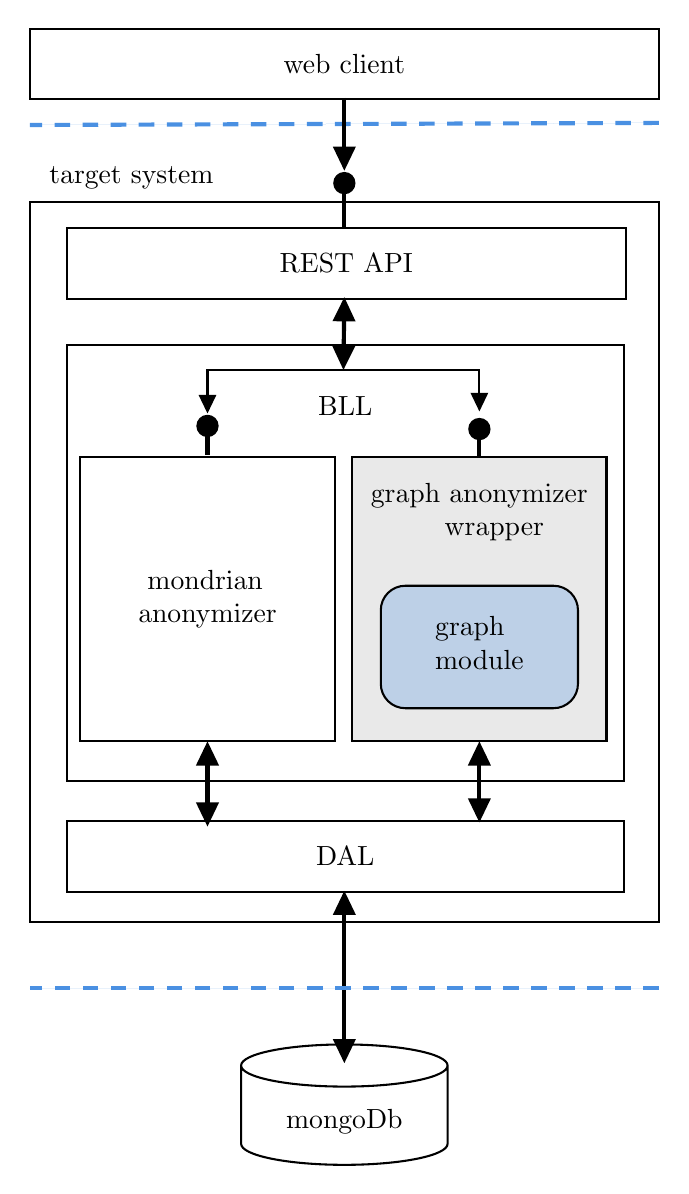
\begin{tikzpicture}[x=0.75pt,y=0.75pt,yscale=-1,xscale=1]
%uncomment if require: \path (0,571); %set diagram left start at 0, and has height of 571

%Shape: Rectangle [id:dp25314219983411235]
\draw  [fill={rgb, 255:red, 155; green, 155; blue, 155 }  ,fill opacity=0.22 ] (349.75,216) -- (472.25,216) -- (472.25,353) -- (349.75,353) -- cycle ;
%Rounded Rect [id:dp6104192131332256]
\draw  [fill={rgb, 255:red, 74; green, 144; blue, 226 }  ,fill opacity=0.28 ] (363.5,289.8) .. controls (363.5,283.28) and (368.78,278) .. (375.3,278) -- (446.7,278) .. controls (453.22,278) and (458.5,283.28) .. (458.5,289.8) -- (458.5,325.2) .. controls (458.5,331.72) and (453.22,337) .. (446.7,337) -- (375.3,337) .. controls (368.78,337) and (363.5,331.72) .. (363.5,325.2) -- cycle ;
%Shape: Rectangle [id:dp7542396041522255]
\draw   (194.38,9.62) -- (497.5,9.62) -- (497.5,43.63) -- (194.38,43.63) -- cycle ;

%Shape: Rectangle [id:dp8775304827751447]
\draw   (194.37,93) -- (497.5,93) -- (497.5,440) -- (194.37,440) -- cycle ;
%Shape: Rectangle [id:dp29329734503174665]
\draw   (212.25,105.63) -- (481.5,105.63) -- (481.5,139.63) -- (212.25,139.63) -- cycle ;

%Shape: Rectangle [id:dp3924156131636001]
\draw   (212.25,162) -- (480.5,162) -- (480.5,372) -- (212.25,372) -- cycle ;
%Shape: Rectangle [id:dp02053336225786917]
\draw   (212.25,391.41) -- (480.5,391.41) -- (480.5,425.41) -- (212.25,425.41) -- cycle ;

%Shape: Rectangle [id:dp8663149504803358]
\draw   (218.75,216) -- (341.25,216) -- (341.25,353) -- (218.75,353) -- cycle ;
%Flowchart: Magnetic Disk [id:dp36269861006508]
\draw   (395.69,509.15) -- (395.69,546.85) .. controls (395.69,552.46) and (373.41,557) .. (345.94,557) .. controls (318.46,557) and (296.19,552.46) .. (296.19,546.85) -- (296.19,509.15)(395.69,509.15) .. controls (395.69,514.76) and (373.41,519.3) .. (345.94,519.3) .. controls (318.46,519.3) and (296.19,514.76) .. (296.19,509.15) .. controls (296.19,503.54) and (318.46,499) .. (345.94,499) .. controls (373.41,499) and (395.69,503.54) .. (395.69,509.15) -- cycle ;

%Straight Lines [id:da08877933566463603]
\draw [color={rgb, 255:red, 74; green, 144; blue, 226 }  ,draw opacity=1 ][fill={rgb, 255:red, 74; green, 144; blue, 226 }  ,fill opacity=1 ][line width=1.5]  [dash pattern={on 5.63pt off 4.5pt}]  (497.5,55) -- (194.38,56) ;


%Straight Lines [id:da5932184702081]
\draw [line width=1.5]    (345.94,84) -- (345.94,105) ;

\draw [shift={(345.94,84)}, rotate = 90] [color={rgb, 255:red, 0; green, 0; blue, 0 }  ][fill={rgb, 255:red, 0; green, 0; blue, 0 }  ][line width=1.5]      (0, 0) circle [x radius= 4.36, y radius= 4.36]   ;
%Straight Lines [id:da8662427461600262]
\draw [line width=1.5]    (345.94,43) -- (345.94,75) ;
\draw [shift={(345.94,78)}, rotate = 270] [fill={rgb, 255:red, 0; green, 0; blue, 0 }  ][line width=1.5]  [draw opacity=0] (11.61,-5.58) -- (0,0) -- (11.61,5.58) -- cycle    ;

%Straight Lines [id:da5790521830826718]
\draw [line width=1.5]    (345.94,428) -- (345.94,505) ;
\draw [shift={(345.94,508)}, rotate = 270] [fill={rgb, 255:red, 0; green, 0; blue, 0 }  ][line width=1.5]  [draw opacity=0] (11.61,-5.58) -- (0,0) -- (11.61,5.58) -- cycle    ;
\draw [shift={(345.94,425)}, rotate = 90] [fill={rgb, 255:red, 0; green, 0; blue, 0 }  ][line width=1.5]  [draw opacity=0] (11.61,-5.58) -- (0,0) -- (11.61,5.58) -- cycle    ;
%Straight Lines [id:da9813732944058937]
\draw [line width=1.5]    (345.9,142) -- (345.54,171) ;
\draw [shift={(345.5,174)}, rotate = 270.72] [fill={rgb, 255:red, 0; green, 0; blue, 0 }  ][line width=1.5]  [draw opacity=0] (11.61,-5.58) -- (0,0) -- (11.61,5.58) -- cycle    ;
\draw [shift={(345.94,139)}, rotate = 90.72] [fill={rgb, 255:red, 0; green, 0; blue, 0 }  ][line width=1.5]  [draw opacity=0] (11.61,-5.58) -- (0,0) -- (11.61,5.58) -- cycle    ;
%Straight Lines [id:da5100456793816999]
\draw [line width=1.5]    (280,356) -- (280,391) ;
\draw [shift={(280,394)}, rotate = 270] [fill={rgb, 255:red, 0; green, 0; blue, 0 }  ][line width=1.5]  [draw opacity=0] (11.61,-5.58) -- (0,0) -- (11.61,5.58) -- cycle    ;
\draw [shift={(280,353)}, rotate = 90] [fill={rgb, 255:red, 0; green, 0; blue, 0 }  ][line width=1.5]  [draw opacity=0] (11.61,-5.58) -- (0,0) -- (11.61,5.58) -- cycle    ;
%Straight Lines [id:da9511987307073959]
\draw [color={rgb, 255:red, 74; green, 144; blue, 226 }  ,draw opacity=1 ][fill={rgb, 255:red, 74; green, 144; blue, 226 }  ,fill opacity=1 ][line width=1.5]  [dash pattern={on 5.63pt off 4.5pt}]  (497.5,472) -- (194.37,472) ;


%Straight Lines [id:da6634746570080241]
\draw [line width=1.5]    (280,201) -- (280,215) ;

\draw [shift={(280,201)}, rotate = 90] [color={rgb, 255:red, 0; green, 0; blue, 0 }  ][fill={rgb, 255:red, 0; green, 0; blue, 0 }  ][line width=1.5]      (0, 0) circle [x radius= 4.36, y radius= 4.36]   ;
%Straight Lines [id:da11396993553443457]
\draw [line width=1.5]    (411,202.5) -- (411,216.5) ;

\draw [shift={(411,202.5)}, rotate = 90] [color={rgb, 255:red, 0; green, 0; blue, 0 }  ][fill={rgb, 255:red, 0; green, 0; blue, 0 }  ][line width=1.5]      (0, 0) circle [x radius= 4.36, y radius= 4.36]   ;
%Straight Lines [id:da6497437274365285]
\draw [line width=1.5]    (411,356) -- (411,389) ;
\draw [shift={(411,392)}, rotate = 270] [fill={rgb, 255:red, 0; green, 0; blue, 0 }  ][line width=1.5]  [draw opacity=0] (11.61,-5.58) -- (0,0) -- (11.61,5.58) -- cycle    ;
\draw [shift={(411,353)}, rotate = 90] [fill={rgb, 255:red, 0; green, 0; blue, 0 }  ][line width=1.5]  [draw opacity=0] (11.61,-5.58) -- (0,0) -- (11.61,5.58) -- cycle    ;
%Straight Lines [id:da30407000837324416]
\draw    (280,193) -- (280,174) -- (411,174) -- (411,192) ;
\draw [shift={(411,194)}, rotate = 270] [fill={rgb, 255:red, 0; green, 0; blue, 0 }  ][line width=0.75]  [draw opacity=0] (8.93,-4.29) -- (0,0) -- (8.93,4.29) -- cycle    ;
\draw [shift={(280,195)}, rotate = 270] [fill={rgb, 255:red, 0; green, 0; blue, 0 }  ][line width=0.75]  [draw opacity=0] (8.93,-4.29) -- (0,0) -- (8.93,4.29) -- cycle    ;

% Text Node
\draw (411,305.5) node [scale=1] [align=left] { graph\\module};
% Text Node
\draw (243.38,81.25) node  [align=left] {target system};
% Text Node
\draw (346.88,122.63) node  [align=left] {REST API};
% Text Node
\draw (346.37,408.41) node  [align=left] {DAL};
% Text Node
\draw (346.38,191.63) node  [align=left] {BLL};
% Text Node
\draw (280,284.5) node  [align=left] { \ mondrian\\anonymizer};
% Text Node
\draw (411,242.63) node  [align=left] {graph anonymizer\\ \ \ \ \ \ \ \ \ wrapper};
% Text Node
\draw (345.94,536) node  [align=left] {mongoDb};
% Text Node
\draw (345.94,26.63) node  [align=left] {web client};


\end{tikzpicture}
    \caption{Integration with the target system}\label{fig:integration_arch}
\end{figure}